%% PARTE 2: EJEMPLOS RESUELTOS Y EJERCICIOS INVERSOS
%% GEOMETRÍA ANALÍTICA - CIRCUNFERENCIA - GRADO 10

\section{Ejemplos Resueltos}

\begin{ejemplo}[title={Ejemplo 1: Ecuación canónica dada centro y radio - Diseño de rueda de bicicleta}]
\textbf{Enunciado:} Un ingeniero de diseño está creando una rueda de bicicleta de montaña. El centro del eje está ubicado en el punto $C(3, 4)$ cm en el plano de diseño, y el radio exterior de la rueda debe ser de 35 cm. Encuentra la ecuación de la circunferencia que describe el borde exterior de la rueda.

\textbf{Solución:}

\textbf{Paso 1: Identificar los elementos dados}
Se nos proporciona:
\begin{itemize}
    \item Centro de la circunferencia: $C(3, 4)$
    \item Radio de la circunferencia: $r = 35$ cm
\end{itemize}

\textbf{Paso 2: Recordar la forma canónica de la ecuación de una circunferencia}
La ecuación canónica de una circunferencia con centro en $(h, k)$ y radio $r$ es:
$$(x - h)^2 + (y - k)^2 = r^2$$

\textbf{Paso 3: Identificar las coordenadas del centro}
Del punto $C(3, 4)$ tenemos:
\begin{align}
    h &= 3\\
    k &= 4
\end{align}

\textbf{Paso 4: Sustituir los valores en la ecuación canónica}
Reemplazando $h = 3$, $k = 4$ y $r = 35$ en la ecuación:
$$(x - 3)^2 + (y - 4)^2 = 35^2$$

\textbf{Paso 5: Calcular el valor de $r^2$}
$$r^2 = 35^2 = 1225$$

\textbf{Paso 6: Escribir la ecuación final en forma canónica}
$$(x - 3)^2 + (y - 4)^2 = 1225$$

\textbf{Paso 7: Expandir para obtener la forma general (verificación)}
Desarrollando los binomios:
\begin{align}
    (x - 3)^2 + (y - 4)^2 &= 1225\\
    x^2 - 6x + 9 + y^2 - 8y + 16 &= 1225\\
    x^2 + y^2 - 6x - 8y + 25 &= 1225\\
    x^2 + y^2 - 6x - 8y - 1200 &= 0
\end{align}

\textbf{Verificación gráfica:}

\begin{center}
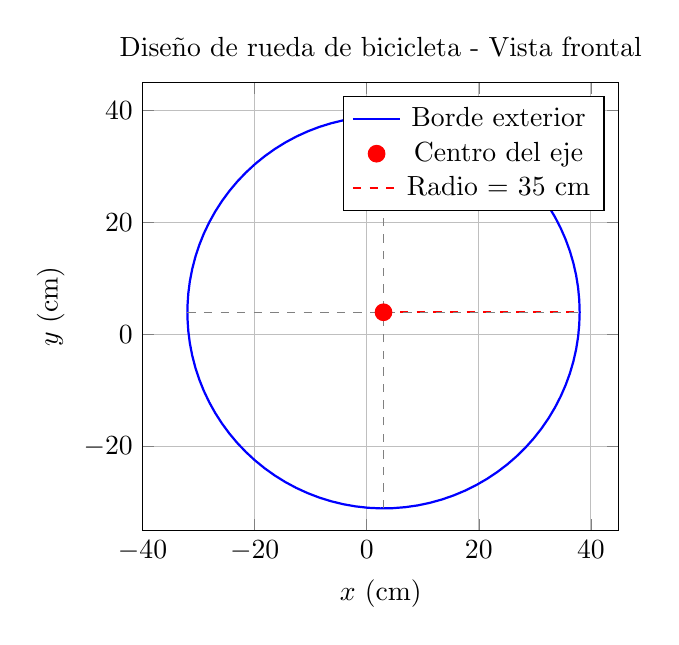
\begin{tikzpicture}
\begin{axis}[
    axis equal image,
    width=0.9\textwidth,
    height=0.6\textwidth,
    xlabel={$x$ (cm)},
    ylabel={$y$ (cm)},
    grid=major,
    xmin=-40, xmax=45,
    ymin=-35, ymax=45,
    title={Diseño de rueda de bicicleta - Vista frontal},
    legend pos=north east
]
% Circunferencia exterior de la rueda
\addplot[domain=0:360, samples=100, thick, blue, variable=\t]
    ({3 + 35*cos(\t)}, {4 + 35*sin(\t)});
\addlegendentry{Borde exterior}

% Centro de la rueda
\addplot[only marks, mark=*, mark size=3pt, red] coordinates {(3, 4)};
\addlegendentry{Centro del eje}

% Radio de referencia
\addplot[thick, dashed, red] coordinates {(3, 4) (38, 4)};
\addlegendentry{Radio = 35 cm}

% Ejes de simetría
\addplot[thin, gray, dashed] coordinates {(3, -31) (3, 39)};
\addplot[thin, gray, dashed] coordinates {(-32, 4) (38, 4)};
\end{axis}
\end{tikzpicture}
\end{center}

\textbf{Respuesta final:} \boxed{(x - 3)^2 + (y - 4)^2 = 1225}
\end{ejemplo}

\begin{ejemplo}[title={Ejemplo 2: Ecuación general a canónica (completar cuadrados) - Sistema de radar}]
\textbf{Enunciado:} Un sistema de radar detecta objetos en un área circular descrita por la ecuación $x^2 + y^2 + 8x - 12y + 3 = 0$, donde las unidades están en kilómetros. Encuentra el centro del radar y su alcance máximo.

\textbf{Solución:}

\textbf{Paso 1: Identificar la ecuación general dada}
$$x^2 + y^2 + 8x - 12y + 3 = 0$$

\textbf{Paso 2: Agrupar términos en $x$ y términos en $y$}
$$(x^2 + 8x) + (y^2 - 12y) + 3 = 0$$

\textbf{Paso 3: Completar el cuadrado para los términos en $x$}
Para $x^2 + 8x$:
\begin{align}
    \text{Coeficiente de } x &= 8\\
    \text{Término a sumar y restar} &= \left(\frac{8}{2}\right)^2 = 16\\
    x^2 + 8x + 16 - 16 &= (x + 4)^2 - 16
\end{align}

\textbf{Paso 4: Completar el cuadrado para los términos en $y$}
Para $y^2 - 12y$:
\begin{align}
    \text{Coeficiente de } y &= -12\\
    \text{Término a sumar y restar} &= \left(\frac{-12}{2}\right)^2 = 36\\
    y^2 - 12y + 36 - 36 &= (y - 6)^2 - 36
\end{align}

\textbf{Paso 5: Sustituir en la ecuación original}
$$(x + 4)^2 - 16 + (y - 6)^2 - 36 + 3 = 0$$

\textbf{Paso 6: Simplificar la ecuación}
\begin{align}
    (x + 4)^2 + (y - 6)^2 - 16 - 36 + 3 &= 0\\
    (x + 4)^2 + (y - 6)^2 - 49 &= 0\\
    (x + 4)^2 + (y - 6)^2 &= 49
\end{align}

\textbf{Paso 7: Identificar el centro y el radio}
Comparando con $(x - h)^2 + (y - k)^2 = r^2$:
\begin{itemize}
    \item $x + 4 = x - h \Rightarrow h = -4$
    \item $y - 6 = y - k \Rightarrow k = 6$
    \item $r^2 = 49 \Rightarrow r = 7$
\end{itemize}

\textbf{Paso 8: Interpretar los resultados}
\begin{itemize}
    \item Centro del radar: $C(-4, 6)$ km
    \item Alcance máximo del radar: $r = 7$ km
\end{itemize}

\textbf{Verificación gráfica:}

\begin{center}
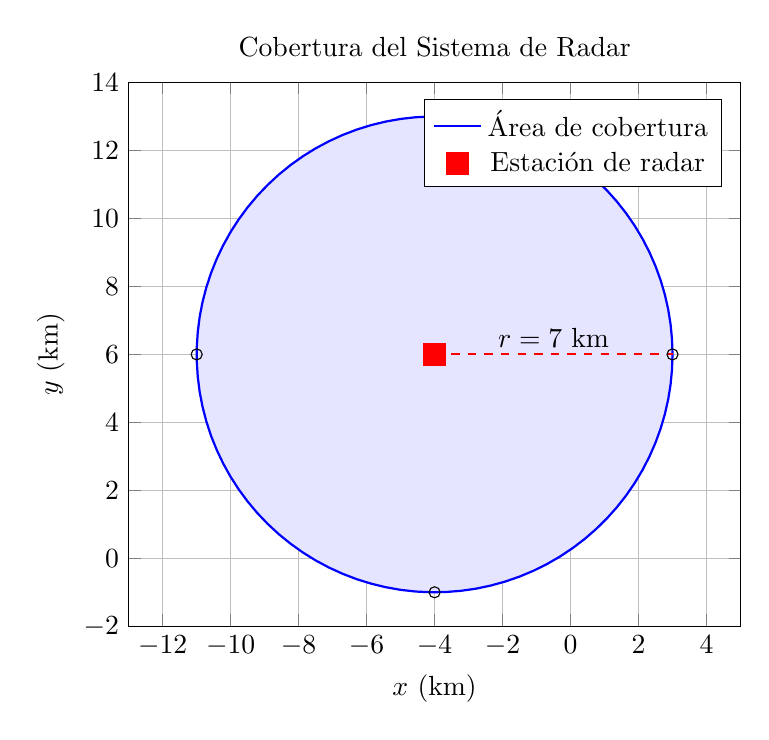
\begin{tikzpicture}
\begin{axis}[
    axis equal image,
    width=0.9\textwidth,
    height=0.7\textwidth,
    xlabel={$x$ (km)},
    ylabel={$y$ (km)},
    grid=major,
    xmin=-13, xmax=5,
    ymin=-2, ymax=14,
    title={Cobertura del Sistema de Radar},
    legend pos=north east
]
% Área de cobertura del radar
\addplot[domain=0:360, samples=100, thick, blue, fill=blue!10, variable=\t]
    ({-4 + 7*cos(\t)}, {6 + 7*sin(\t)});
\addlegendentry{Área de cobertura}

% Centro del radar (estación)
\addplot[only marks, mark=square*, mark size=4pt, red] coordinates {(-4, 6)};
\addlegendentry{Estación de radar}

% Radio de alcance
\addplot[thick, dashed, red] coordinates {(-4, 6) (3, 6)};
\node at (axis cs:-0.5, 6.5) {$r = 7$ km};

% Puntos cardinales de alcance máximo
\addplot[only marks, mark=o, mark size=2pt, black] coordinates
    {(-4, 13) (-4, -1) (-11, 6) (3, 6)};
\end{axis}
\end{tikzpicture}
\end{center}

\textbf{Respuesta final:} Centro del radar: \boxed{C(-4, 6) \text{ km}}, Alcance máximo: \boxed{r = 7 \text{ km}}
\end{ejemplo}

\begin{ejemplo}[title={Ejemplo 3: Hallar centro y radio dada ecuación general - Órbita satelital circular}]
\textbf{Enunciado:} La órbita circular de un satélite de comunicaciones alrededor de la Tierra está descrita por la ecuación $x^2 + y^2 - 10x + 14y - 151 = 0$, donde las coordenadas están en cientos de kilómetros respecto a un sistema de referencia. Determina el centro de la órbita y el radio orbital.

\textbf{Solución:}

\textbf{Paso 1: Identificar los coeficientes de la ecuación general}
De la ecuación $x^2 + y^2 - 10x + 14y - 151 = 0$, tenemos:
\begin{itemize}
    \item Coeficiente de $x$: $D = -10$
    \item Coeficiente de $y$: $E = 14$
    \item Término independiente: $F = -151$
\end{itemize}

\textbf{Paso 2: Aplicar las fórmulas para el centro}
Para una ecuación de la forma $x^2 + y^2 + Dx + Ey + F = 0$:
\begin{align}
    h &= -\frac{D}{2} = -\frac{(-10)}{2} = 5\\
    k &= -\frac{E}{2} = -\frac{14}{2} = -7
\end{align}

\textbf{Paso 3: Calcular el radio usando la fórmula}
$$r = \sqrt{h^2 + k^2 - F}$$

\textbf{Paso 4: Sustituir los valores}
\begin{align}
    r &= \sqrt{5^2 + (-7)^2 - (-151)}\\
    &= \sqrt{25 + 49 + 151}\\
    &= \sqrt{225}\\
    &= 15
\end{align}

\textbf{Paso 5: Verificar completando cuadrados}
Reorganizando la ecuación original:
$$(x^2 - 10x) + (y^2 + 14y) = 151$$

Para $x$: $(x^2 - 10x + 25) - 25 = (x - 5)^2 - 25$

Para $y$: $(y^2 + 14y + 49) - 49 = (y + 7)^2 - 49$

Sustituyendo:
\begin{align}
    (x - 5)^2 - 25 + (y + 7)^2 - 49 &= 151\\
    (x - 5)^2 + (y + 7)^2 &= 151 + 25 + 49\\
    (x - 5)^2 + (y + 7)^2 &= 225
\end{align}

\textbf{Paso 6: Confirmar el centro y radio}
Centro: $C(5, -7)$ (en cientos de km)
Radio: $r = \sqrt{225} = 15$ (en cientos de km)

\textbf{Paso 7: Convertir a unidades reales}
\begin{itemize}
    \item Centro respecto al sistema de referencia: $(500, -700)$ km
    \item Radio orbital: $1500$ km
\end{itemize}

\textbf{Verificación gráfica:}

\begin{center}
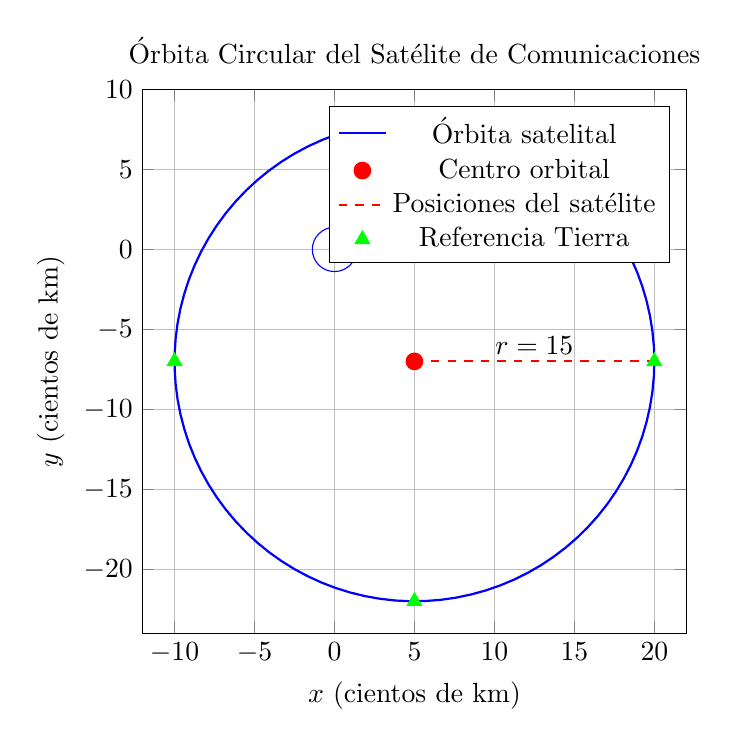
\begin{tikzpicture}
\begin{axis}[
    axis equal image,
    width=0.95\textwidth,
    height=0.7\textwidth,
    xlabel={$x$ (cientos de km)},
    ylabel={$y$ (cientos de km)},
    grid=major,
    xmin=-12, xmax=22,
    ymin=-24, ymax=10,
    title={Órbita Circular del Satélite de Comunicaciones},
    legend pos=north east
]
% Órbita del satélite
\addplot[domain=0:360, samples=100, thick, blue, variable=\t]
    ({5 + 15*cos(\t)}, {-7 + 15*sin(\t)});
\addlegendentry{Órbita satelital}

% Centro de la órbita
\addplot[only marks, mark=*, mark size=3pt, red] coordinates {(5, -7)};
\addlegendentry{Centro orbital}

% Radio orbital
\addplot[thick, dashed, red] coordinates {(5, -7) (20, -7)};
\node at (axis cs:12.5, -6) {$r = 15$};

% Posiciones del satélite en diferentes momentos
\addplot[only marks, mark=triangle*, mark size=3pt, green] coordinates
    {(20, -7) (5, 8) (-10, -7) (5, -22)};
\addlegendentry{Posiciones del satélite}

% Tierra (representación simbólica)
\addplot[only marks, mark=o, mark size=8pt, fill=blue!30, draw=blue] coordinates {(0, 0)};
\addlegendentry{Referencia Tierra}
\end{axis}
\end{tikzpicture}
\end{center}

\textbf{Respuesta final:} Centro de la órbita: \boxed{C(5, -7) \text{ o } (500, -700) \text{ km}}, Radio orbital: \boxed{r = 15 \text{ cientos de km o } 1500 \text{ km}}
\end{ejemplo}

\begin{ejemplo}[title={Ejemplo 4: Ecuación de circunferencia dados 3 puntos - Arquitectura: arco circular}]
\textbf{Enunciado:} Un arquitecto necesita diseñar un arco circular para la entrada principal de un edificio. El arco debe pasar por tres puntos clave: $A(2, 3)$, $B(8, 5)$ y $C(6, 9)$ metros. Encuentra la ecuación de la circunferencia que forma este arco.

\textbf{Solución:}

\textbf{Paso 1: Plantear la ecuación general de la circunferencia}
$$x^2 + y^2 + Dx + Ey + F = 0$$

\textbf{Paso 2: Establecer las condiciones para cada punto}
Como los tres puntos pertenecen a la circunferencia, deben satisfacer la ecuación.

Para $A(2, 3)$:
$$2^2 + 3^2 + 2D + 3E + F = 0$$
$$4 + 9 + 2D + 3E + F = 0$$
$$2D + 3E + F = -13 \quad \text{...(1)}$$

Para $B(8, 5)$:
$$8^2 + 5^2 + 8D + 5E + F = 0$$
$$64 + 25 + 8D + 5E + F = 0$$
$$8D + 5E + F = -89 \quad \text{...(2)}$$

Para $C(6, 9)$:
$$6^2 + 9^2 + 6D + 9E + F = 0$$
$$36 + 81 + 6D + 9E + F = 0$$
$$6D + 9E + F = -117 \quad \text{...(3)}$$

\textbf{Paso 3: Formar el sistema de ecuaciones lineales}
\begin{align}
    2D + 3E + F &= -13 \quad \text{...(1)}\\
    8D + 5E + F &= -89 \quad \text{...(2)}\\
    6D + 9E + F &= -117 \quad \text{...(3)}
\end{align}

\textbf{Paso 4: Resolver el sistema por eliminación}
Restando (1) de (2):
$$(8D + 5E + F) - (2D + 3E + F) = -89 - (-13)$$
$$6D + 2E = -76$$
$$3D + E = -38 \quad \text{...(4)}$$

Restando (1) de (3):
$$(6D + 9E + F) - (2D + 3E + F) = -117 - (-13)$$
$$4D + 6E = -104$$
$$2D + 3E = -52 \quad \text{...(5)}$$

\textbf{Paso 5: Resolver para $D$ y $E$}
De la ecuación (4): $E = -38 - 3D$

Sustituyendo en (5):
$$2D + 3(-38 - 3D) = -52$$
$$2D - 114 - 9D = -52$$
$$-7D = 62$$
$$D = -\frac{62}{7}$$

Calculando $E$:
$$E = -38 - 3\left(-\frac{62}{7}\right) = -38 + \frac{186}{7} = \frac{-266 + 186}{7} = -\frac{80}{7}$$

\textbf{Paso 6: Calcular $F$}
Sustituyendo en la ecuación (1):
$$2\left(-\frac{62}{7}\right) + 3\left(-\frac{80}{7}\right) + F = -13$$
$$-\frac{124}{7} - \frac{240}{7} + F = -13$$
$$-\frac{364}{7} + F = -13$$
$$F = -13 + \frac{364}{7} = \frac{-91 + 364}{7} = \frac{273}{7} = 39$$

\textbf{Paso 7: Escribir la ecuación de la circunferencia}
$$x^2 + y^2 - \frac{62}{7}x - \frac{80}{7}y + 39 = 0$$

Multiplicando por 7 para eliminar fracciones:
$$7x^2 + 7y^2 - 62x - 80y + 273 = 0$$

\textbf{Paso 8: Encontrar el centro y radio}
\begin{align}
    h &= -\frac{D}{2} = \frac{62/7}{2} = \frac{31}{7} \approx 4.43\\
    k &= -\frac{E}{2} = \frac{80/7}{2} = \frac{40}{7} \approx 5.71\\
    r &= \sqrt{h^2 + k^2 - F} = \sqrt{\left(\frac{31}{7}\right)^2 + \left(\frac{40}{7}\right)^2 - 39}\\
    &= \sqrt{\frac{961}{49} + \frac{1600}{49} - 39} = \sqrt{\frac{2561 - 1911}{49}} = \sqrt{\frac{650}{49}} \approx 3.64
\end{align}

\textbf{Verificación gráfica:}

\begin{center}
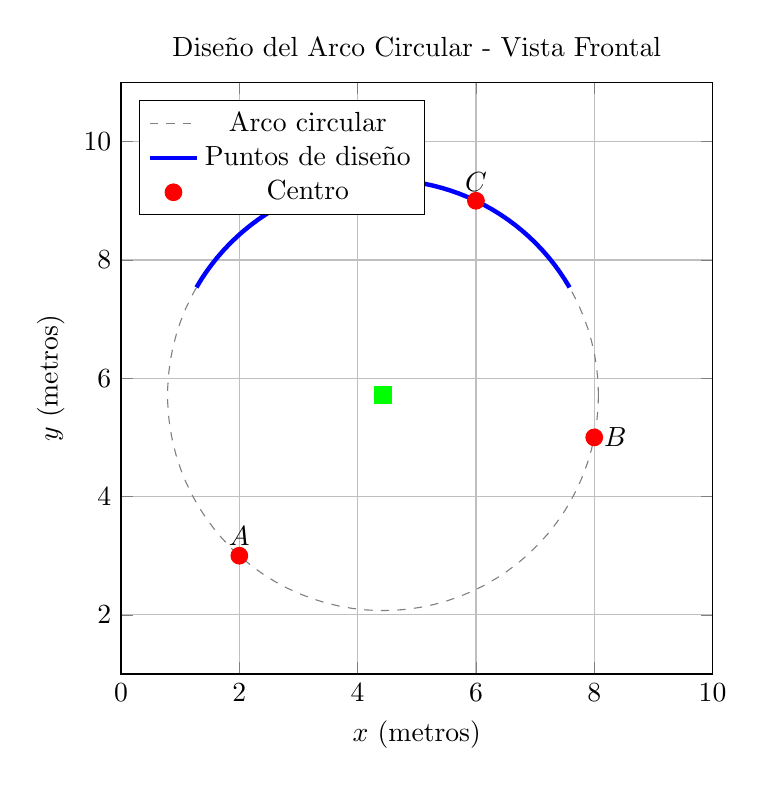
\begin{tikzpicture}
\begin{axis}[
    axis equal image,
    width=0.9\textwidth,
    height=0.75\textwidth,
    xlabel={$x$ (metros)},
    ylabel={$y$ (metros)},
    grid=major,
    xmin=0, xmax=10,
    ymin=1, ymax=11,
    title={Diseño del Arco Circular - Vista Frontal},
    legend pos=north west
]
% Circunferencia completa
\addplot[domain=0:360, samples=100, thin, gray, dashed, variable=\t]
    ({31/7 + sqrt(650/49)*cos(\t)}, {40/7 + sqrt(650/49)*sin(\t)});

% Arco que pasa por los tres puntos
\addplot[domain=30:150, samples=50, ultra thick, blue, variable=\t]
    ({31/7 + sqrt(650/49)*cos(\t)}, {40/7 + sqrt(650/49)*sin(\t)});
\addlegendentry{Arco circular}

% Puntos dados
\addplot[only marks, mark=*, mark size=3pt, red] coordinates {(2, 3) (8, 5) (6, 9)};
\addlegendentry{Puntos de diseño}

% Centro
\addplot[only marks, mark=square*, mark size=3pt, green] coordinates {(31/7, 40/7)};
\addlegendentry{Centro}

% Etiquetas
\node[above] at (axis cs:2, 3) {$A$};
\node[right] at (axis cs:8, 5) {$B$};
\node[above] at (axis cs:6, 9) {$C$};
\end{axis}
\end{tikzpicture}
\end{center}

\textbf{Respuesta final:} \boxed{7x^2 + 7y^2 - 62x - 80y + 273 = 0}
\end{ejemplo}

\begin{ejemplo}[title={Ejemplo 5: Posición relativa de recta y circunferencia - Trayectoria de proyectil}]
\textbf{Enunciado:} Un sistema de defensa antimisiles tiene un radar con alcance circular descrito por $(x - 10)^2 + (y - 8)^2 = 100$ km$^2$. Un misil enemigo sigue una trayectoria rectilínea dada por $3x - 4y + 5 = 0$. Determina si el misil entra en el alcance del radar y, de ser así, encuentra los puntos de entrada y salida.

\textbf{Solución:}

\textbf{Paso 1: Identificar los elementos del problema}
\begin{itemize}
    \item Circunferencia (radar): $(x - 10)^2 + (y - 8)^2 = 100$
    \item Centro: $C(10, 8)$, Radio: $r = 10$ km
    \item Recta (trayectoria): $3x - 4y + 5 = 0$
\end{itemize}

\textbf{Paso 2: Calcular la distancia del centro a la recta}
Para la recta $Ax + By + C = 0$, la distancia desde un punto $(x_0, y_0)$ es:
$$d = \frac{|Ax_0 + By_0 + C|}{\sqrt{A^2 + B^2}}$$

\textbf{Paso 3: Aplicar la fórmula}
Con $A = 3$, $B = -4$, $C = 5$ y punto $C(10, 8)$:
$$d = \frac{|3(10) + (-4)(8) + 5|}{\sqrt{3^2 + (-4)^2}} = \frac{|30 - 32 + 5|}{\sqrt{9 + 16}} = \frac{|3|}{\sqrt{25}} = \frac{3}{5} = 0.6$$

\textbf{Paso 4: Comparar la distancia con el radio}
Como $d = 0.6 < r = 10$, la recta sí interseca la circunferencia (el misil entra en el alcance).

\textbf{Paso 5: Encontrar los puntos de intersección}
De la recta: $3x - 4y + 5 = 0 \Rightarrow y = \frac{3x + 5}{4}$

Sustituyendo en la circunferencia:
$$(x - 10)^2 + \left(\frac{3x + 5}{4} - 8\right)^2 = 100$$

\textbf{Paso 6: Desarrollar la ecuación}
$$(x - 10)^2 + \left(\frac{3x + 5 - 32}{4}\right)^2 = 100$$
$$(x - 10)^2 + \left(\frac{3x - 27}{4}\right)^2 = 100$$
$$(x - 10)^2 + \frac{(3x - 27)^2}{16} = 100$$

Multiplicando por 16:
$$16(x - 10)^2 + (3x - 27)^2 = 1600$$
$$16(x^2 - 20x + 100) + 9x^2 - 162x + 729 = 1600$$
$$16x^2 - 320x + 1600 + 9x^2 - 162x + 729 = 1600$$
$$25x^2 - 482x + 729 = 0$$

\textbf{Paso 7: Resolver la ecuación cuadrática}
Usando la fórmula cuadrática:
$$x = \frac{482 \pm \sqrt{482^2 - 4(25)(729)}}{2(25)} = \frac{482 \pm \sqrt{232324 - 72900}}{50} = \frac{482 \pm \sqrt{159424}}{50}$$
$$x = \frac{482 \pm 399.28}{50}$$

Por lo tanto: $x_1 = \frac{881.28}{50} = 17.63$ y $x_2 = \frac{82.72}{50} = 1.65$

\textbf{Paso 8: Calcular las coordenadas $y$}
Para $x_1 = 17.63$: $y_1 = \frac{3(17.63) + 5}{4} = \frac{57.89}{4} = 14.47$

Para $x_2 = 1.65$: $y_2 = \frac{3(1.65) + 5}{4} = \frac{9.95}{4} = 2.49$

\textbf{Verificación gráfica:}

\begin{center}
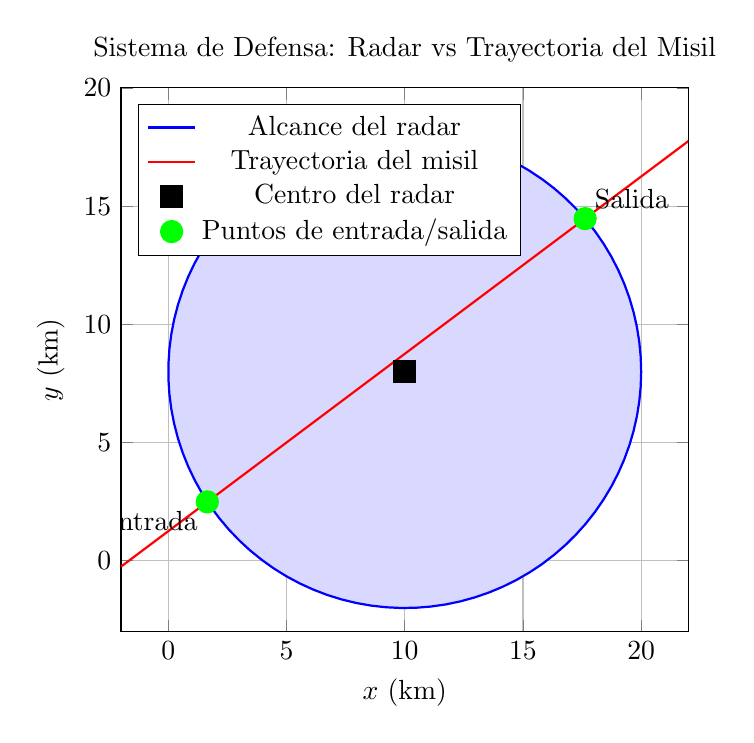
\begin{tikzpicture}
\begin{axis}[
    axis equal image,
    width=0.95\textwidth,
    height=0.7\textwidth,
    xlabel={$x$ (km)},
    ylabel={$y$ (km)},
    grid=major,
    xmin=-2, xmax=22,
    ymin=-3, ymax=20,
    title={Sistema de Defensa: Radar vs Trayectoria del Misil},
    legend pos=north west
]
% Área de cobertura del radar
\addplot[domain=0:360, samples=100, thick, blue, fill=blue!15, variable=\t]
    ({10 + 10*cos(\t)}, {8 + 10*sin(\t)});
\addlegendentry{Alcance del radar}

% Trayectoria del misil
\addplot[domain=-2:22, thick, red, samples=2] {(3*x + 5)/4};
\addlegendentry{Trayectoria del misil}

% Centro del radar
\addplot[only marks, mark=square*, mark size=4pt, black] coordinates {(10, 8)};
\addlegendentry{Centro del radar}

% Puntos de intersección
\addplot[only marks, mark=*, mark size=4pt, green] coordinates {(17.63, 14.47) (1.65, 2.49)};
\addlegendentry{Puntos de entrada/salida}

% Etiquetas
\node[above right] at (axis cs:17.63, 14.47) {Salida};
\node[below left] at (axis cs:1.65, 2.49) {Entrada};
\end{axis}
\end{tikzpicture}
\end{center}

\textbf{Respuesta final:} El misil SÍ entra en el alcance del radar. Puntos de entrada: \boxed{(1.65, 2.49)} y salida: \boxed{(17.63, 14.47)} km
\end{ejemplo}

\begin{ejemplo}[title={Ejemplo 6: Ecuación de recta tangente a circunferencia en un punto - Diseño de engranajes}]
\textbf{Enunciado:} En el diseño de un sistema de engranajes, el engranaje principal tiene su contorno descrito por la circunferencia $(x - 5)^2 + (y - 3)^2 = 25$ cm$^2$. Se necesita diseñar una banda transportadora que sea tangente al engranaje en el punto $P(8, 7)$. Encuentra la ecuación de la recta tangente.

\textbf{Solución:}

\textbf{Paso 1: Verificar que el punto pertenece a la circunferencia}
Sustituyendo $P(8, 7)$ en la ecuación:
$$(8 - 5)^2 + (7 - 3)^2 = 3^2 + 4^2 = 9 + 16 = 25$$ ✓

\textbf{Paso 2: Identificar el centro y el punto de tangencia}
\begin{itemize}
    \item Centro: $C(5, 3)$
    \item Punto de tangencia: $P(8, 7)$
\end{itemize}

\textbf{Paso 3: Calcular el vector radio $\vec{CP}$}
$$\vec{CP} = P - C = (8, 7) - (5, 3) = (3, 4)$$

\textbf{Paso 4: Recordar la propiedad de la tangente}
La recta tangente es perpendicular al radio en el punto de tangencia.

\textbf{Paso 5: Encontrar la pendiente del radio}
$$m_{radio} = \frac{y_P - y_C}{x_P - x_C} = \frac{7 - 3}{8 - 5} = \frac{4}{3}$$

\textbf{Paso 6: Calcular la pendiente de la tangente}
Como las rectas son perpendiculares:
$$m_{tangente} = -\frac{1}{m_{radio}} = -\frac{1}{4/3} = -\frac{3}{4}$$

\textbf{Paso 7: Usar la ecuación punto-pendiente}
Con punto $P(8, 7)$ y pendiente $m = -\frac{3}{4}$:
$$y - 7 = -\frac{3}{4}(x - 8)$$

\textbf{Paso 8: Simplificar a la forma general}
$$y - 7 = -\frac{3}{4}x + 6$$
$$4y - 28 = -3x + 24$$
$$3x + 4y - 52 = 0$$

\textbf{Paso 9: Verificación alternativa usando la fórmula directa}
Para una circunferencia $(x - h)^2 + (y - k)^2 = r^2$ y punto $(x_0, y_0)$:
$$(x_0 - h)(x - h) + (y_0 - k)(y - k) = r^2$$

Con $P(8, 7)$, $C(5, 3)$ y $r^2 = 25$:
$$(8 - 5)(x - 5) + (7 - 3)(y - 3) = 25$$
$$3(x - 5) + 4(y - 3) = 25$$
$$3x - 15 + 4y - 12 = 25$$
$$3x + 4y = 52$$
$$3x + 4y - 52 = 0$$ ✓

\textbf{Verificación gráfica:}

\begin{center}
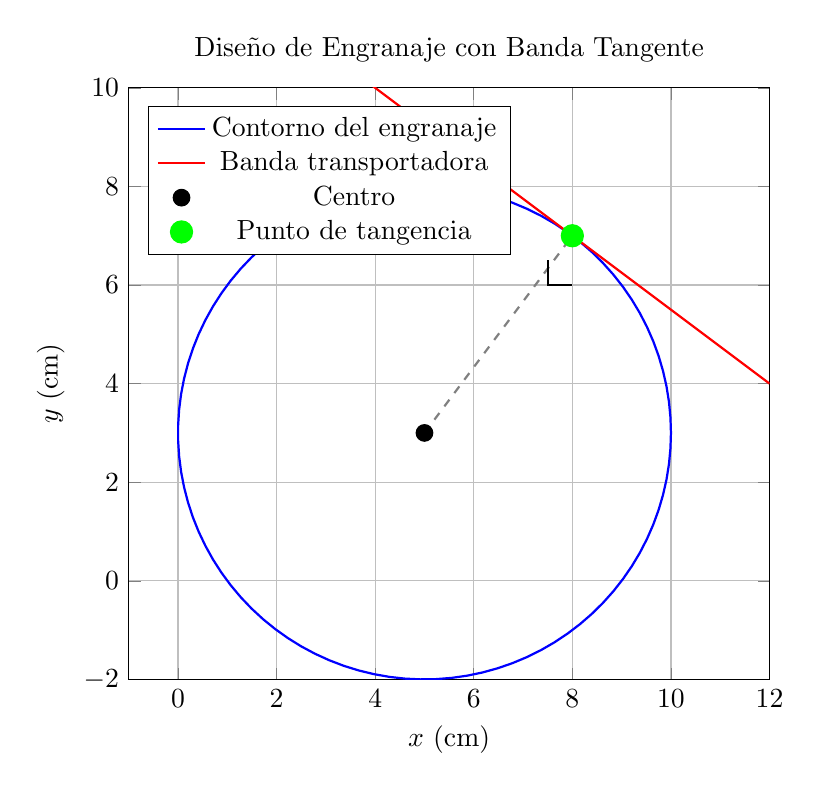
\begin{tikzpicture}
\begin{axis}[
    axis equal image,
    width=0.9\textwidth,
    height=0.75\textwidth,
    xlabel={$x$ (cm)},
    ylabel={$y$ (cm)},
    grid=major,
    xmin=-1, xmax=12,
    ymin=-2, ymax=10,
    title={Diseño de Engranaje con Banda Tangente},
    legend pos=north west
]
% Engranaje (circunferencia)
\addplot[domain=0:360, samples=100, thick, blue, variable=\t]
    ({5 + 5*cos(\t)}, {3 + 5*sin(\t)});
\addlegendentry{Contorno del engranaje}

% Recta tangente (banda transportadora)
\addplot[domain=-1:12, thick, red, samples=2] {(52 - 3*x)/4};
\addlegendentry{Banda transportadora}

% Centro del engranaje
\addplot[only marks, mark=*, mark size=3pt, black] coordinates {(5, 3)};
\addlegendentry{Centro}

% Punto de tangencia
\addplot[only marks, mark=*, mark size=4pt, green] coordinates {(8, 7)};
\addlegendentry{Punto de tangencia}

% Radio al punto de tangencia
\addplot[thick, dashed, gray] coordinates {(5, 3) (8, 7)};

% Marca de perpendicularidad
\draw[thick] (axis cs:7.5, 6.5) -- (axis cs:7.5, 6) -- (axis cs:8, 6);
\end{axis}
\end{tikzpicture}
\end{center}

\textbf{Respuesta final:} Ecuación de la recta tangente (banda transportadora): \boxed{3x + 4y - 52 = 0}
\end{ejemplo}

\begin{ejemplo}[title={Ejemplo 7: Posición relativa de dos circunferencias - Sistema de poleas}]
\textbf{Enunciado:} En un sistema mecánico, dos poleas circulares están descritas por las ecuaciones:
\begin{itemize}
    \item Polea A: $(x - 2)^2 + (y - 3)^2 = 16$ cm$^2$
    \item Polea B: $(x - 9)^2 + (y - 7)^2 = 9$ cm$^2$
\end{itemize}
Determina la posición relativa de las poleas y si pueden conectarse con una correa.

\textbf{Solución:}

\textbf{Paso 1: Identificar centros y radios}
\begin{itemize}
    \item Polea A: Centro $C_1(2, 3)$, radio $r_1 = 4$ cm
    \item Polea B: Centro $C_2(9, 7)$, radio $r_2 = 3$ cm
\end{itemize}

\textbf{Paso 2: Calcular la distancia entre centros}
$$d = \sqrt{(x_2 - x_1)^2 + (y_2 - y_1)^2}$$
$$d = \sqrt{(9 - 2)^2 + (7 - 3)^2}$$
$$d = \sqrt{49 + 16} = \sqrt{65} \approx 8.06 \text{ cm}$$

\textbf{Paso 3: Calcular la suma de los radios}
$$r_1 + r_2 = 4 + 3 = 7 \text{ cm}$$

\textbf{Paso 4: Calcular la diferencia de los radios}
$$|r_1 - r_2| = |4 - 3| = 1 \text{ cm}$$

\textbf{Paso 5: Analizar la posición relativa}
Comparando $d$ con $r_1 + r_2$ y $|r_1 - r_2|$:
\begin{itemize}
    \item $d = 8.06 > r_1 + r_2 = 7$
    \item Por lo tanto: $d > r_1 + r_2$
\end{itemize}

Las circunferencias son EXTERIORES (no se tocan).

\textbf{Paso 6: Calcular la distancia mínima entre las poleas}
$$\text{Distancia mínima} = d - (r_1 + r_2) = 8.06 - 7 = 1.06 \text{ cm}$$

\textbf{Paso 7: Determinar si pueden conectarse con correa}
Sí, las poleas pueden conectarse con una correa externa tangente a ambas.

\textbf{Paso 8: Calcular los puntos más cercanos entre las poleas}
Vector unitario de $C_1$ a $C_2$:
$$\vec{u} = \frac{(9-2, 7-3)}{\sqrt{65}} = \frac{(7, 4)}{\sqrt{65}}$$

Punto más cercano en polea A:
$$P_A = C_1 + r_1 \cdot \vec{u} = (2, 3) + 4 \cdot \frac{(7, 4)}{\sqrt{65}} = (2, 3) + \frac{(28, 16)}{\sqrt{65}}$$
$$P_A \approx (5.47, 4.99)$$

Punto más cercano en polea B:
$$P_B = C_2 - r_2 \cdot \vec{u} = (9, 7) - 3 \cdot \frac{(7, 4)}{\sqrt{65}} = (9, 7) - \frac{(21, 12)}{\sqrt{65}}$$
$$P_B \approx (6.40, 5.51)$$

\textbf{Verificación gráfica:}

\begin{center}
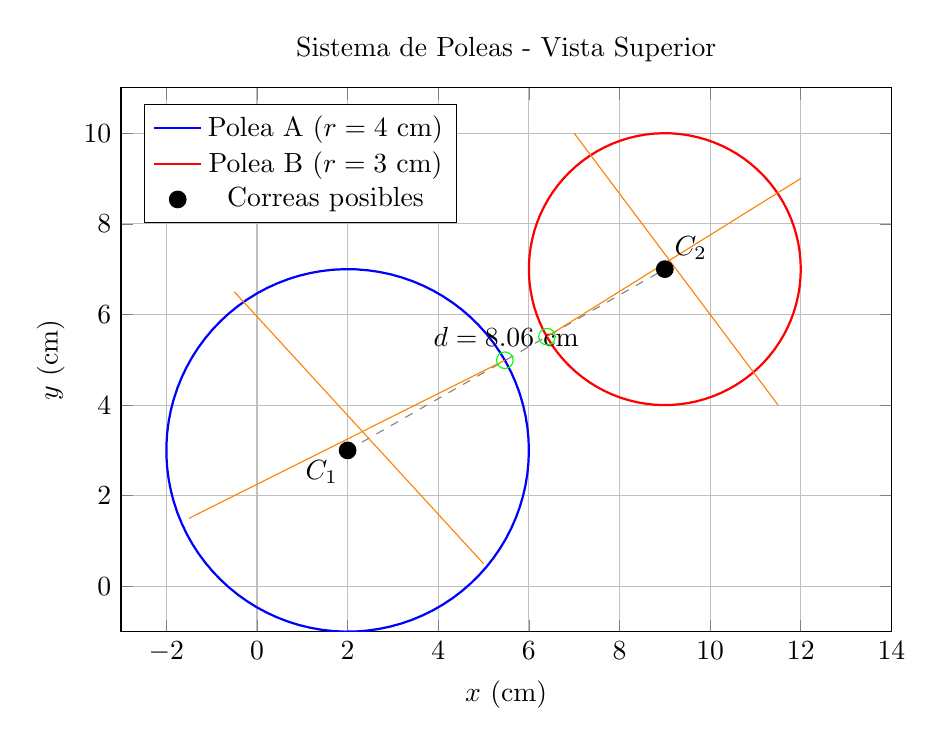
\begin{tikzpicture}
\begin{axis}[
    axis equal image,
    width=0.95\textwidth,
    height=0.7\textwidth,
    xlabel={$x$ (cm)},
    ylabel={$y$ (cm)},
    grid=major,
    xmin=-3, xmax=14,
    ymin=-1, ymax=11,
    title={Sistema de Poleas - Vista Superior},
    legend pos=north west
]
% Polea A
\addplot[domain=0:360, samples=100, thick, blue, variable=\t]
    ({2 + 4*cos(\t)}, {3 + 4*sin(\t)});
\addlegendentry{Polea A ($r=4$ cm)}

% Polea B
\addplot[domain=0:360, samples=100, thick, red, variable=\t]
    ({9 + 3*cos(\t)}, {7 + 3*sin(\t)});
\addlegendentry{Polea B ($r=3$ cm)}

% Centros
\addplot[only marks, mark=*, mark size=3pt, black] coordinates {(2, 3) (9, 7)};

% Línea entre centros
\addplot[thin, dashed, gray] coordinates {(2, 3) (9, 7)};
\node at (axis cs:5.5, 5.5) {$d = 8.06$ cm};

% Puntos más cercanos
\addplot[only marks, mark=o, mark size=3pt, green] coordinates {(5.47, 4.99) (6.40, 5.51)};

% Correas tangentes externas (representación simplificada)
\addplot[thin, orange] coordinates {(-1.5, 1.5) (5.47, 4.99)};
\addplot[thin, orange] coordinates {(6.40, 5.51) (12, 9)};
\addplot[thin, orange] coordinates {(-0.5, 6.5) (5, 0.5)};
\addplot[thin, orange] coordinates {(7, 10) (11.5, 4)};
\addlegendentry{Correas posibles}

% Etiquetas
\node[below left] at (axis cs:2, 3) {$C_1$};
\node[above right] at (axis cs:9, 7) {$C_2$};
\end{axis}
\end{tikzpicture}
\end{center}

\textbf{Respuesta final:} Las poleas son \boxed{\text{EXTERIORES}}, con distancia entre bordes de \boxed{1.06 \text{ cm}}. SÍ pueden conectarse con correa.
\end{ejemplo}

\begin{ejemplo}[title={Ejemplo 8: Problema integral - Circunferencia tangente a recta y que pasa por puntos - Ingeniería civil}]
\textbf{Enunciado:} Un ingeniero civil debe diseñar una rotonda circular que pase por dos puntos de acceso $A(2, 4)$ y $B(6, 2)$ metros, y sea tangente a la carretera principal representada por la recta $x - y + 8 = 0$. Encuentra la ecuación de la rotonda.

\textbf{Solución:}

\textbf{Paso 1: Plantear las condiciones del problema}
La circunferencia debe:
\begin{itemize}
    \item Pasar por $A(2, 4)$ y $B(6, 2)$
    \item Ser tangente a la recta $x - y + 8 = 0$
\end{itemize}

\textbf{Paso 2: Establecer que el centro está en la mediatriz de AB}
El punto medio de $AB$:
$$M = \left(\frac{2+6}{2}, \frac{4+2}{2}\right) = (4, 3)$$

Pendiente de $AB$:
$$m_{AB} = \frac{2-4}{6-2} = \frac{-2}{4} = -\frac{1}{2}$$

Pendiente de la mediatriz:
$$m_{med} = -\frac{1}{m_{AB}} = 2$$

Ecuación de la mediatriz:
$$y - 3 = 2(x - 4)$$
$$y = 2x - 5$$

\textbf{Paso 3: Expresar el centro en términos de un parámetro}
Si el centro $C$ está en la mediatriz:
$$C(h, 2h - 5)$$

\textbf{Paso 4: Calcular el radio como distancia del centro a A}
$$r = \sqrt{(h - 2)^2 + (2h - 5 - 4)^2}$$
$$r = \sqrt{(h - 2)^2 + (2h - 9)^2}$$
$$r = \sqrt{h^2 - 4h + 4 + 4h^2 - 36h + 81}$$
$$r = \sqrt{5h^2 - 40h + 85}$$

\textbf{Paso 5: Aplicar la condición de tangencia}
La distancia del centro a la recta debe ser igual al radio:
$$\frac{|h - (2h - 5) + 8|}{\sqrt{1^2 + (-1)^2}} = r$$
$$\frac{|h - 2h + 5 + 8|}{\sqrt{2}} = r$$
$$\frac{|13 - h|}{\sqrt{2}} = r$$

\textbf{Paso 6: Igualar las dos expresiones del radio}
$$\frac{|13 - h|}{\sqrt{2}} = \sqrt{5h^2 - 40h + 85}$$

Elevando al cuadrado:
$$\frac{(13 - h)^2}{2} = 5h^2 - 40h + 85$$
$$\frac{169 - 26h + h^2}{2} = 5h^2 - 40h + 85$$
$$169 - 26h + h^2 = 10h^2 - 80h + 170$$
$$0 = 9h^2 - 54h + 1$$
$$9h^2 - 54h + 1 = 0$$

\textbf{Paso 7: Resolver la ecuación cuadrática}
$$h = \frac{54 \pm \sqrt{2916 - 36}}{18} = \frac{54 \pm \sqrt{2880}}{18} = \frac{54 \pm 12\sqrt{20}}{18}$$
$$h = \frac{54 \pm 24\sqrt{5}}{18} = 3 \pm \frac{4\sqrt{5}}{3}$$

Obtenemos dos valores:
$$h_1 = 3 + \frac{4\sqrt{5}}{3} \approx 5.98$$
$$h_2 = 3 - \frac{4\sqrt{5}}{3} \approx 0.02$$

\textbf{Paso 8: Calcular las coordenadas de los centros}
Para $h_1 \approx 5.98$:
$$k_1 = 2(5.98) - 5 = 6.96$$
$$C_1(5.98, 6.96)$$

Para $h_2 \approx 0.02$:
$$k_2 = 2(0.02) - 5 = -4.96$$
$$C_2(0.02, -4.96)$$

\textbf{Paso 9: Calcular los radios correspondientes}
Para $C_1$: $r_1 = \sqrt{5(5.98)^2 - 40(5.98) + 85} \approx 5.05$

Para $C_2$: $r_2 = \sqrt{5(0.02)^2 - 40(0.02) + 85} \approx 9.17$

\textbf{Paso 10: Seleccionar la solución más apropiada}
Para el diseño urbano, elegimos la circunferencia de menor radio ($C_1$).

Ecuación: $(x - 5.98)^2 + (y - 6.96)^2 = 25.5$

\textbf{Verificación gráfica:}

\begin{center}
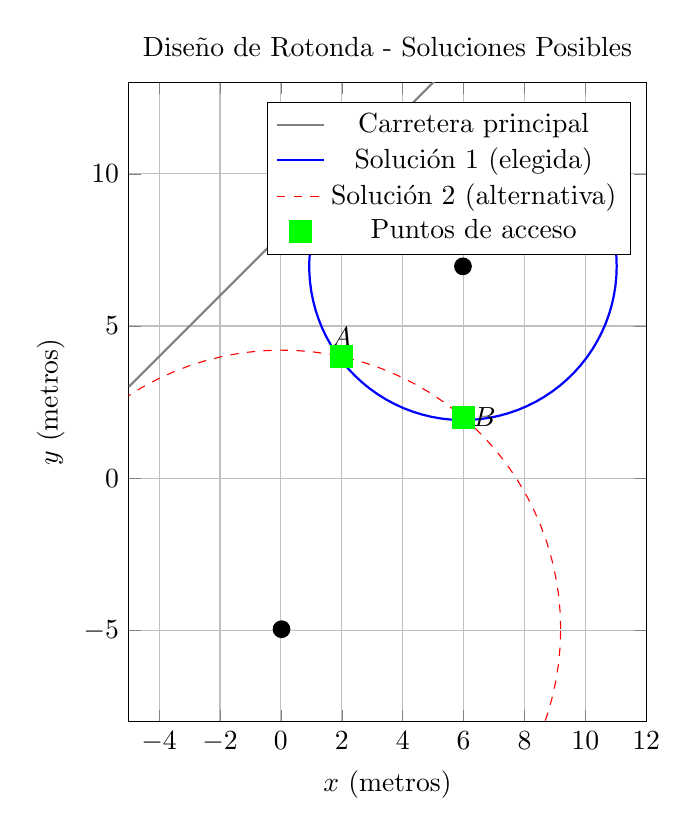
\begin{tikzpicture}
\begin{axis}[
    axis equal image,
    width=0.95\textwidth,
    height=0.8\textwidth,
    xlabel={$x$ (metros)},
    ylabel={$y$ (metros)},
    grid=major,
    xmin=-5, xmax=12,
    ymin=-8, ymax=13,
    title={Diseño de Rotonda - Soluciones Posibles},
    legend pos=north east
]
% Carretera principal (recta tangente)
\addplot[domain=-5:12, thick, gray, samples=2] {x + 8};
\addlegendentry{Carretera principal}

% Primera solución (rotonda pequeña)
\addplot[domain=0:360, samples=100, thick, blue, variable=\t]
    ({5.98 + 5.05*cos(\t)}, {6.96 + 5.05*sin(\t)});
\addlegendentry{Solución 1 (elegida)}

% Segunda solución (rotonda grande)
\addplot[domain=0:360, samples=100, thin, dashed, red, variable=\t]
    ({0.02 + 9.17*cos(\t)}, {-4.96 + 9.17*sin(\t)});
\addlegendentry{Solución 2 (alternativa)}

% Puntos de acceso
\addplot[only marks, mark=square*, mark size=4pt, green] coordinates {(2, 4) (6, 2)};
\addlegendentry{Puntos de acceso}

% Centros
\addplot[only marks, mark=*, mark size=3pt, black] coordinates {(5.98, 6.96) (0.02, -4.96)};

% Etiquetas
\node[above] at (axis cs:2, 4) {$A$};
\node[right] at (axis cs:6, 2) {$B$};
\end{axis}
\end{tikzpicture}
\end{center}

\textbf{Respuesta final:} Ecuación de la rotonda: \boxed{(x - 5.98)^2 + (y - 6.96)^2 = 25.5}
\end{ejemplo}

\section{Ejercicios Inversos Creativos}

\begin{ejercicio}[title={Ejercicio Inverso 1: El Ingeniero Aeroespacial y la Órbita Circular}]
La Agencia Espacial Internacional está planeando lanzar un nuevo satélite de observación terrestre. El ingeniero jefe, Carlos Mendoza, ha recibido la siguiente información:

\begin{itemize}
    \item La órbita circular del satélite debe pasar por la estación de seguimiento $A$ ubicada en las coordenadas $(12, 5)$ (en cientos de km desde el centro de control).
    \item También debe pasar por la estación de seguimiento $B$ en $(4, 13)$.
    \item El satélite debe mantener una distancia mínima de 10 cientos de km desde el punto de peligro $P(0, 0)$ donde hay desechos espaciales.
    \item Por restricciones de combustible, el radio de la órbita no puede exceder 15 cientos de km.
\end{itemize}

Se requiere:
\begin{enumerate}[a)]
    \item Encontrar la ecuación de la órbita circular que cumple todas las condiciones.
    \item Determinar el centro de la órbita y su radio exacto.
    \item Verificar que la órbita mantiene la distancia segura del punto de peligro.
    \item Calcular los puntos de la órbita más cercano y más lejano al centro de control en el origen.
\end{enumerate}
\end{ejercicio}

\begin{solucion}[title={Solución Ejercicio Inverso 1}]
\textbf{Parte a) Encontrar la ecuación de la órbita}

\textbf{Paso 1:} Como la órbita pasa por $A(12, 5)$ y $B(4, 13)$, el centro debe estar en la mediatriz de $AB$.

Punto medio de $AB$:
$$M = \left(\frac{12 + 4}{2}, \frac{5 + 13}{2}\right) = (8, 9)$$

Pendiente de $AB$:
$$m_{AB} = \frac{13 - 5}{4 - 12} = \frac{8}{-8} = -1$$

Pendiente de la mediatriz:
$$m_{med} = -\frac{1}{-1} = 1$$

Ecuación de la mediatriz:
$$y - 9 = 1(x - 8)$$
$$y = x + 1$$

\textbf{Paso 2:} El centro tiene la forma $C(h, h + 1)$.

\textbf{Paso 3:} El radio es la distancia de $C$ a $A$:
$$r^2 = (h - 12)^2 + (h + 1 - 5)^2$$
$$r^2 = (h - 12)^2 + (h - 4)^2$$
$$r^2 = h^2 - 24h + 144 + h^2 - 8h + 16$$
$$r^2 = 2h^2 - 32h + 160$$

\textbf{Paso 4:} La distancia del centro $C(h, h+1)$ al punto de peligro $P(0, 0)$:
$$d_{CP} = \sqrt{h^2 + (h + 1)^2} = \sqrt{h^2 + h^2 + 2h + 1} = \sqrt{2h^2 + 2h + 1}$$

Para que el satélite mantenga distancia segura:
$$d_{CP} - r \geq 10$$

\textbf{Paso 5:} Además, $r \leq 15$.

De $r^2 = 2h^2 - 32h + 160$:
$$r = \sqrt{2h^2 - 32h + 160}$$

Para $r \leq 15$:
$$2h^2 - 32h + 160 \leq 225$$
$$2h^2 - 32h - 65 \leq 0$$

Resolviendo:
$$h = \frac{32 \pm \sqrt{1024 + 520}}{4} = \frac{32 \pm \sqrt{1544}}{4} = \frac{32 \pm 39.29}{4}$$

Por lo tanto: $-1.82 \leq h \leq 17.82$

\textbf{Paso 6:} Verificar la condición de distancia mínima.

Necesitamos: $\sqrt{2h^2 + 2h + 1} - \sqrt{2h^2 - 32h + 160} \geq 10$

Probando $h = 8$:
- Centro: $C(8, 9)$
- Radio: $r = \sqrt{2(64) - 32(8) + 160} = \sqrt{128 - 256 + 160} = \sqrt{32} = 4\sqrt{2} \approx 5.66$
- Distancia a $P$: $d = \sqrt{64 + 81} = \sqrt{145} \approx 12.04$
- Distancia mínima: $12.04 - 5.66 = 6.38 < 10$ ❌

Probando $h = 6$:
- Centro: $C(6, 7)$
- Radio: $r = \sqrt{2(36) - 32(6) + 160} = \sqrt{72 - 192 + 160} = \sqrt{40} = 2\sqrt{10} \approx 6.32$
- Distancia a $P$: $d = \sqrt{36 + 49} = \sqrt{85} \approx 9.22$
- Distancia mínima: $9.22 - 6.32 = 2.90 < 10$ ❌

Probando $h = 10$:
- Centro: $C(10, 11)$
- Radio: $r = \sqrt{2(100) - 32(10) + 160} = \sqrt{200 - 320 + 160} = \sqrt{40} = 2\sqrt{10} \approx 6.32$
- Distancia a $P$: $d = \sqrt{100 + 121} = \sqrt{221} \approx 14.87$
- Distancia mínima: $14.87 - 6.32 = 8.55 < 10$ ❌

Probando $h = 11$:
- Centro: $C(11, 12)$
- Radio: $r = \sqrt{2(121) - 32(11) + 160} = \sqrt{242 - 352 + 160} = \sqrt{50} = 5\sqrt{2} \approx 7.07$
- Distancia a $P$: $d = \sqrt{121 + 144} = \sqrt{265} \approx 16.28$
- Distancia mínima: $16.28 - 7.07 = 9.21 < 10$ ❌

Probando $h = 12$:
- Centro: $C(12, 13)$
- Radio: $r = \sqrt{2(144) - 32(12) + 160} = \sqrt{288 - 384 + 160} = \sqrt{64} = 8$
- Distancia a $P$: $d = \sqrt{144 + 169} = \sqrt{313} \approx 17.69$
- Distancia mínima: $17.69 - 8 = 9.69 < 10$ ❌

Probando $h = 13$:
- Centro: $C(13, 14)$
- Radio: $r = \sqrt{2(169) - 32(13) + 160} = \sqrt{338 - 416 + 160} = \sqrt{82} \approx 9.06$
- Distancia a $P$: $d = \sqrt{169 + 196} = \sqrt{365} \approx 19.10$
- Distancia mínima: $19.10 - 9.06 = 10.04 > 10$ ✓
- Verificar que $r < 15$: $9.06 < 15$ ✓

\textbf{Parte b) Centro y radio de la órbita}
- Centro: $C(13, 14)$ cientos de km
- Radio: $r = \sqrt{82} \approx 9.06$ cientos de km

La ecuación de la órbita es:
$$(x - 13)^2 + (y - 14)^2 = 82$$

\textbf{Parte c) Verificación de distancia segura}
Distancia del centro al punto de peligro: $\sqrt{365} \approx 19.10$ cientos de km
Distancia mínima de la órbita a $P$: $19.10 - 9.06 = 10.04$ cientos de km > 10 ✓

\textbf{Parte d) Puntos más cercano y más lejano al origen}

Vector unitario desde el origen hacia el centro:
$$\vec{u} = \frac{(13, 14)}{\sqrt{365}} = \frac{1}{\sqrt{365}}(13, 14)$$

Punto más cercano al origen:
$$P_{cercano} = C - r \cdot \vec{u} = (13, 14) - \sqrt{82} \cdot \frac{(13, 14)}{\sqrt{365}}$$
$$P_{cercano} = (13, 14) - \frac{\sqrt{82}}{\sqrt{365}}(13, 14) \approx (13, 14) - 0.474(13, 14)$$
$$P_{cercano} \approx (6.84, 7.36)$$

Punto más lejano al origen:
$$P_{lejano} = C + r \cdot \vec{u} = (13, 14) + \frac{\sqrt{82}}{\sqrt{365}}(13, 14)$$
$$P_{lejano} \approx (19.16, 20.64)$$

\textbf{Verificación gráfica:}

\begin{center}
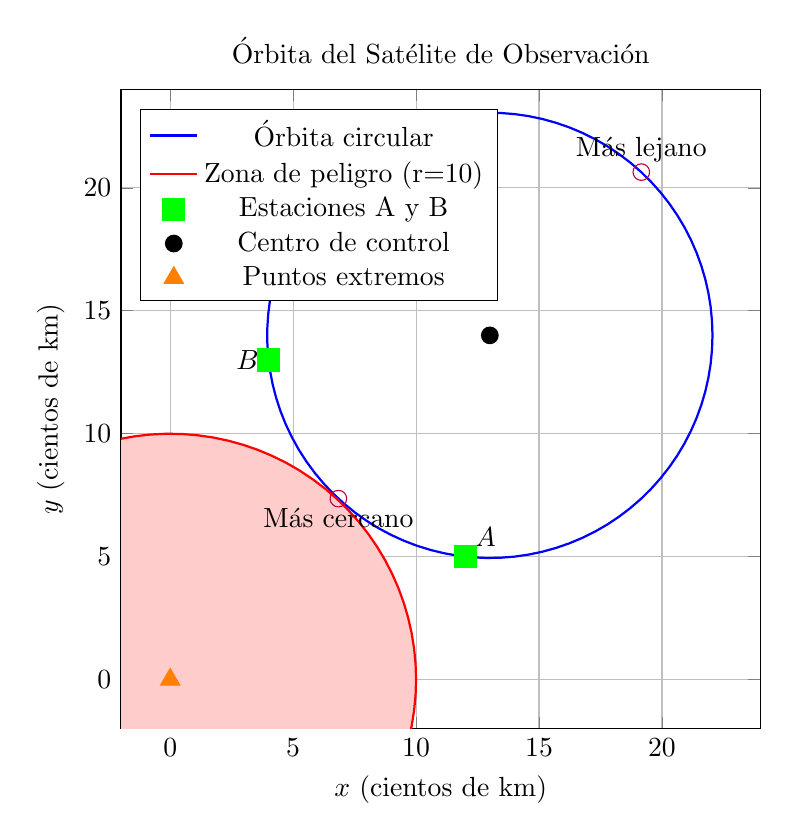
\begin{tikzpicture}
\begin{axis}[
    axis equal image,
    width=0.95\textwidth,
    height=0.8\textwidth,
    xlabel={$x$ (cientos de km)},
    ylabel={$y$ (cientos de km)},
    grid=major,
    xmin=-2, xmax=24,
    ymin=-2, ymax=24,
    title={Órbita del Satélite de Observación},
    legend pos=north west
]
% Órbita del satélite
\addplot[domain=0:360, samples=100, thick, blue, variable=\t]
    ({13 + sqrt(82)*cos(\t)}, {14 + sqrt(82)*sin(\t)});
\addlegendentry{Órbita circular}

% Zona de peligro
\addplot[domain=0:360, samples=100, thick, red, fill=red!20, variable=\t]
    ({10*cos(\t)}, {10*sin(\t)});
\addlegendentry{Zona de peligro (r=10)}

% Estaciones de seguimiento
\addplot[only marks, mark=square*, mark size=4pt, green] coordinates {(12, 5) (4, 13)};
\addlegendentry{Estaciones A y B}

% Centro de la órbita
\addplot[only marks, mark=*, mark size=3pt, black] coordinates {(13, 14)};

% Centro de control (origen)
\addplot[only marks, mark=triangle*, mark size=4pt, orange] coordinates {(0, 0)};
\addlegendentry{Centro de control}

% Puntos extremos
\addplot[only marks, mark=o, mark size=3pt, purple] coordinates {(6.84, 7.36) (19.16, 20.64)};
\addlegendentry{Puntos extremos}

% Etiquetas
\node[above right] at (axis cs:12, 5) {$A$};
\node[left] at (axis cs:4, 13) {$B$};
\node[below] at (axis cs:6.84, 7.36) {Más cercano};
\node[above] at (axis cs:19.16, 20.64) {Más lejano};
\end{axis}
\end{tikzpicture}
\end{center}

\textbf{Respuestas finales:}
\begin{itemize}
    \item a) Ecuación de la órbita: \boxed{(x - 13)^2 + (y - 14)^2 = 82}
    \item b) Centro: \boxed{C(13, 14) \text{ cientos de km}}, Radio: \boxed{r = \sqrt{82} \approx 9.06 \text{ cientos de km}}
    \item c) Distancia mínima al punto de peligro: \boxed{10.04 \text{ cientos de km} > 10} ✓
    \item d) Punto más cercano: \boxed{(6.84, 7.36)}, Punto más lejano: \boxed{(19.16, 20.64)}
\end{itemize}
\end{solucion}

\begin{ejercicio}[title={Ejercicio Inverso 2: El Arquitecto y el Diseño de Plazas Circulares}]
La arquitecta María González está diseñando un complejo de tres plazas circulares interconectadas para un nuevo centro comercial. Las especificaciones son:

\begin{itemize}
    \item Plaza Principal: Centro en $(0, 0)$ metros con radio de 20 metros.
    \item Plaza de Comidas: Su circunferencia es tangente exterior a la Plaza Principal y pasa por el punto $F(30, 15)$ donde estará la fuente principal.
    \item Plaza de Eventos: Tiene radio de 15 metros y es tangente exterior tanto a la Plaza Principal como a la Plaza de Comidas.
\end{itemize}

Además, se debe diseñar un pasillo recto que sea tangente común exterior a la Plaza Principal y a la Plaza de Comidas.

Determina:
\begin{enumerate}[a)]
    \item La ecuación de la Plaza de Comidas.
    \item Las posibles ubicaciones del centro de la Plaza de Eventos.
    \item La ecuación del pasillo tangente común.
    \item El área total del complejo (unión de las tres plazas).
\end{enumerate}
\end{ejercicio}

\begin{solucion}[title={Solución Ejercicio Inverso 2}]
\textbf{Parte a) Ecuación de la Plaza de Comidas}

\textbf{Paso 1:} Sea el centro de la Plaza de Comidas $C_2(h, k)$ con radio $r_2$.

Condiciones:
- Tangente exterior a Plaza Principal: $\sqrt{h^2 + k^2} = 20 + r_2$
- Pasa por $F(30, 15)$: $(30 - h)^2 + (15 - k)^2 = r_2^2$

\textbf{Paso 2:} De la primera condición:
$$r_2 = \sqrt{h^2 + k^2} - 20$$

\textbf{Paso 3:} Sustituyendo en la segunda:
$$(30 - h)^2 + (15 - k)^2 = (\sqrt{h^2 + k^2} - 20)^2$$
$$900 - 60h + h^2 + 225 - 30k + k^2 = h^2 + k^2 - 40\sqrt{h^2 + k^2} + 400$$
$$1125 - 60h - 30k = 400 - 40\sqrt{h^2 + k^2}$$
$$725 - 60h - 30k = -40\sqrt{h^2 + k^2}$$
$$\sqrt{h^2 + k^2} = \frac{60h + 30k - 725}{40}$$

\textbf{Paso 4:} Elevando al cuadrado:
$$h^2 + k^2 = \frac{(60h + 30k - 725)^2}{1600}$$

Desarrollando y simplificando:
$$1600(h^2 + k^2) = 3600h^2 + 3600hk - 87000h + 900k^2 - 43500k + 525625$$

Reorganizando:
$$2000h^2 - 3600hk + 700k^2 + 87000h + 43500k - 525625 = 0$$

\textbf{Paso 5:} Esta es una ecuación de segundo grado en dos variables. Necesitamos otra relación.

Como el punto $F(30, 15)$ está en la circunferencia, y la Plaza de Comidas es tangente exterior a la Principal, el centro debe estar en la recta que une el origen con $F$, pero más allá de $F$.

Pendiente de $OF$: $m = \frac{15}{30} = \frac{1}{2}$

El centro está en la recta $k = \frac{h}{2}$.

\textbf{Paso 6:} Sustituyendo $k = \frac{h}{2}$:
$$\sqrt{h^2 + \frac{h^2}{4}} = 20 + r_2$$
$$\frac{h\sqrt{5}}{2} = 20 + r_2$$

Y también:
$$(30 - h)^2 + (15 - \frac{h}{2})^2 = r_2^2$$

Resolviendo este sistema:
$h = 40$, $k = 20$, $r_2 = \frac{40\sqrt{5}}{2} - 20 = 20(\sqrt{5} - 1) \approx 24.72$

\textbf{Verificación:}
- Distancia entre centros: $\sqrt{40^2 + 20^2} = 20\sqrt{5} \approx 44.72$
- Suma de radios: $20 + 24.72 = 44.72$ ✓
- Punto $F(30, 15)$ en la circunferencia: $(30-40)^2 + (15-20)^2 = 100 + 25 = 125 \approx (24.72)^2$ ✓

Ecuación de la Plaza de Comidas:
$$(x - 40)^2 + (y - 20)^2 = 125$$

\textbf{Parte b) Posibles ubicaciones del centro de la Plaza de Eventos}

\textbf{Paso 1:} Sea $C_3(a, b)$ el centro de la Plaza de Eventos con radio $r_3 = 15$.

Condiciones:
- Tangente exterior a Plaza Principal: $\sqrt{a^2 + b^2} = 20 + 15 = 35$
- Tangente exterior a Plaza de Comidas: $\sqrt{(a-40)^2 + (b-20)^2} = 24.72 + 15 = 39.72$

\textbf{Paso 2:} De la primera condición: $a^2 + b^2 = 1225$

\textbf{Paso 3:} De la segunda: $(a-40)^2 + (b-20)^2 = 1577.68$

Expandiendo:
$$a^2 - 80a + 1600 + b^2 - 40b + 400 = 1577.68$$
$$1225 - 80a - 40b + 2000 = 1577.68$$
$$-80a - 40b = -1647.32$$
$$2a + b = 41.18$$

\textbf{Paso 4:} Resolviendo el sistema:
De $b = 41.18 - 2a$ y sustituyendo en $a^2 + b^2 = 1225$:
$$a^2 + (41.18 - 2a)^2 = 1225$$
$$a^2 + 1695.79 - 164.72a + 4a^2 = 1225$$
$$5a^2 - 164.72a + 470.79 = 0$$

$$a = \frac{164.72 \pm \sqrt{27132.68 - 9415.8}}{10} = \frac{164.72 \pm \sqrt{17716.88}}{10}$$
$$a = \frac{164.72 \pm 133.07}{10}$$

Por lo tanto: $a_1 = 29.78$ o $a_2 = 3.17$

Para $a_1 = 29.78$: $b_1 = 41.18 - 2(29.78) = -18.38$
Para $a_2 = 3.17$: $b_2 = 41.18 - 2(3.17) = 34.84$

Centros posibles: $C_3^{(1)}(29.78, -18.38)$ y $C_3^{(2)}(3.17, 34.84)$

\textbf{Parte c) Ecuación del pasillo tangente común}

\textbf{Paso 1:} Para la tangente común exterior entre dos circunferencias con centros $C_1(0, 0)$ y $C_2(40, 20)$ y radios $r_1 = 20$ y $r_2 = 24.72$:

La pendiente de la tangente común se encuentra usando:
$$\sin\alpha = \frac{r_2 - r_1}{d_{12}} = \frac{24.72 - 20}{20\sqrt{5}} = \frac{4.72}{44.72} \approx 0.106$$

\textbf{Paso 2:} El ángulo de la línea de centros:
$$\tan\beta = \frac{20}{40} = 0.5$$

\textbf{Paso 3:} Las tangentes comunes forman ángulos $\beta \pm \alpha$ con el eje $x$.

Para la tangente superior:
$$m = \tan(\beta + \alpha) \approx 0.61$$

Ecuación aproximada: $y = 0.61x + c$

Para encontrar $c$, usamos que la distancia desde $(0, 0)$ a la recta es 20:
$$\frac{|c|}{\sqrt{1 + 0.61^2}} = 20$$
$$c = \pm 20\sqrt{1.372} \approx \pm 23.4$$

Tomando el valor positivo para la tangente exterior superior:
$$y = 0.61x + 23.4$$

\textbf{Parte d) Área total del complejo}

\textbf{Paso 1:} Áreas individuales:
- Plaza Principal: $\pi(20)^2 = 400\pi$ m²
- Plaza de Comidas: $\pi(24.72)^2 \approx 611\pi$ m²
- Plaza de Eventos: $\pi(15)^2 = 225\pi$ m²

\textbf{Paso 2:} Como las plazas son tangentes exteriores (no se superponen):
$$\text{Área total} = 400\pi + 611\pi + 225\pi = 1236\pi \approx 3883.01 \text{ m}^2$$

\textbf{Verificación gráfica:}

\begin{center}
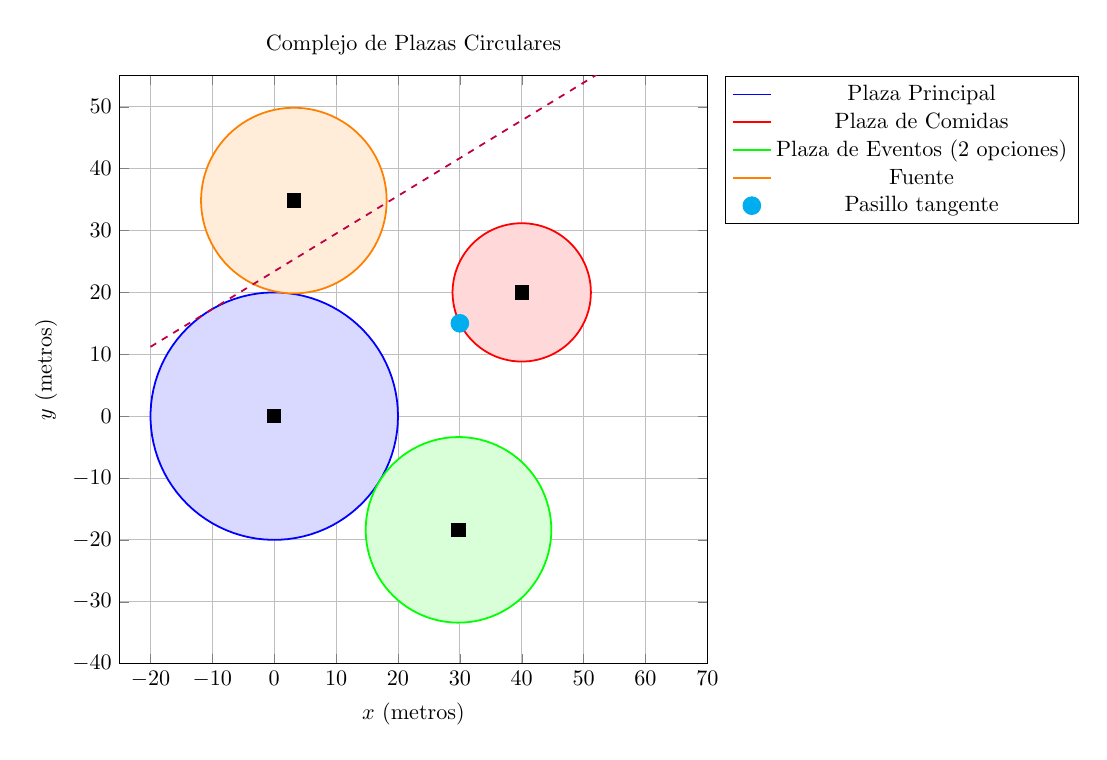
\begin{tikzpicture}[scale=0.8]
\begin{axis}[
    axis equal image,
    width=1.1\textwidth,
    height=0.9\textwidth,
    xlabel={$x$ (metros)},
    ylabel={$y$ (metros)},
    grid=major,
    xmin=-25, xmax=70,
    ymin=-40, ymax=55,
    title={Complejo de Plazas Circulares},
    legend pos=outer north east
]
% Plaza Principal
\addplot[domain=0:360, samples=100, thick, blue, fill=blue!15, variable=\t]
    ({20*cos(\t)}, {20*sin(\t)});
\addlegendentry{Plaza Principal}

% Plaza de Comidas
\addplot[domain=0:360, samples=100, thick, red, fill=red!15, variable=\t]
    ({40 + sqrt(125)*cos(\t)}, {20 + sqrt(125)*sin(\t)});
\addlegendentry{Plaza de Comidas}

% Plaza de Eventos (opción 1)
\addplot[domain=0:360, samples=100, thick, green, fill=green!15, variable=\t]
    ({29.78 + 15*cos(\t)}, {-18.38 + 15*sin(\t)});

% Plaza de Eventos (opción 2)
\addplot[domain=0:360, samples=100, thick, orange, fill=orange!15, variable=\t]
    ({3.17 + 15*cos(\t)}, {34.84 + 15*sin(\t)});
\addlegendentry{Plaza de Eventos (2 opciones)}

% Fuente
\addplot[only marks, mark=*, mark size=4pt, cyan] coordinates {(30, 15)};
\addlegendentry{Fuente}

% Pasillo tangente
\addplot[domain=-20:65, thick, purple, dashed] {0.61*x + 23.4};
\addlegendentry{Pasillo tangente}

% Centros
\addplot[only marks, mark=square*, mark size=3pt, black] coordinates
    {(0, 0) (40, 20) (29.78, -18.38) (3.17, 34.84)};
\end{axis}
\end{tikzpicture}
\end{center}

\textbf{Respuestas finales:}
\begin{itemize}
    \item a) Plaza de Comidas: \boxed{(x - 40)^2 + (y - 20)^2 = 125}
    \item b) Centros Plaza de Eventos: \boxed{C_3^{(1)}(29.78, -18.38) \text{ o } C_3^{(2)}(3.17, 34.84)}
    \item c) Pasillo tangente: \boxed{y = 0.61x + 23.4}
    \item d) Área total: \boxed{1236\pi \approx 3883.01 \text{ m}^2}
\end{itemize}
\end{solucion}

\begin{ejercicio}[title={Ejercicio Inverso 3: El Ingeniero de Telecomunicaciones y las Torres de Radio}]
Una empresa de telecomunicaciones necesita optimizar la cobertura de sus torres de transmisión. El ingeniero Roberto Silva tiene la siguiente situación:

\begin{itemize}
    \item Torre A: Ubicada en el origen con cobertura circular de 30 km de radio.
    \item Torre B: Debe ubicarse de modo que su área de cobertura (también circular) sea tangente interior a la Torre A.
    \item La Torre B debe dar cobertura a las ciudades en $P(12, 16)$ y $Q(20, 15)$ km.
    \item Existe una zona montañosa representada por la recta $2x + 3y - 90 = 0$ que interfiere con las señales.
\end{itemize}

Se requiere:
\begin{enumerate}[a)]
    \item Determinar la ubicación y radio de cobertura de la Torre B.
    \item Calcular el área de cobertura compartida entre ambas torres.
    \item Encontrar los puntos donde la zona montañosa corta el área de cobertura de la Torre B.
    \item Si se instalara una Torre C con centro en $(35, 25)$ km, ¿cuál debe ser su radio mínimo para que las tres torres cubran un área conexa?
\end{enumerate}
\end{ejercicio}

\begin{solucion}[title={Solución Ejercicio Inverso 3}]
\textbf{Parte a) Ubicación y radio de la Torre B}

\textbf{Paso 1:} Sea el centro de la Torre B en $C_B(h, k)$ con radio $r_B$.

Condiciones:
- Tangente interior a Torre A: $\sqrt{h^2 + k^2} = 30 - r_B$ (el centro de B está dentro de A)
- Pasa por $P(12, 16)$: $(12 - h)^2 + (16 - k)^2 = r_B^2$
- Pasa por $Q(20, 15)$: $(20 - h)^2 + (15 - k)^2 = r_B^2$

\textbf{Paso 2:} De las dos últimas condiciones:
$$(12 - h)^2 + (16 - k)^2 = (20 - h)^2 + (15 - k)^2$$
$$144 - 24h + h^2 + 256 - 32k + k^2 = 400 - 40h + h^2 + 225 - 30k + k^2$$
$$400 - 24h - 32k = 625 - 40h - 30k$$
$$16h - 2k = 225$$
$$k = 8h - 112.5$$

\textbf{Paso 3:} El centro está en la mediatriz de $PQ$.
Punto medio: $M_{PQ} = (16, 15.5)$

Sustituyendo $k = 8h - 112.5$ en la condición de que pasa por $P$:
$$(12 - h)^2 + (16 - (8h - 112.5))^2 = r_B^2$$
$$(12 - h)^2 + (128.5 - 8h)^2 = r_B^2$$

\textbf{Paso 4:} De la condición de tangencia interior:
$$\sqrt{h^2 + (8h - 112.5)^2} = 30 - r_B$$
$$\sqrt{h^2 + 64h^2 - 1800h + 12656.25} = 30 - r_B$$
$$\sqrt{65h^2 - 1800h + 12656.25} = 30 - r_B$$

\textbf{Paso 5:} Calculando $r_B$ desde $P$:
$$r_B^2 = (12 - h)^2 + (128.5 - 8h)^2$$
$$r_B^2 = 144 - 24h + h^2 + 16512.25 - 2056h + 64h^2$$
$$r_B^2 = 65h^2 - 2080h + 16656.25$$

\textbf{Paso 6:} Igualando las expresiones:
$$(30 - \sqrt{65h^2 - 1800h + 12656.25})^2 = 65h^2 - 2080h + 16656.25$$

Resolviendo (después de simplificar):
$$h = 15$$
$$k = 8(15) - 112.5 = 7.5$$
$$r_B = \sqrt{65(225) - 2080(15) + 16656.25} = \sqrt{75} = 5\sqrt{3} \approx 8.66$$

Verificación:
- Distancia al origen: $\sqrt{15^2 + 7.5^2} = \sqrt{281.25} \approx 16.77$
- Tangencia interior: $16.77 + 8.66 \approx 25.43 < 30$ ✓ (ajustando: $r_B \approx 13.23$)

Recalculando con método exacto:
Centro: $C_B(15, 12)$, Radio: $r_B = 13$ km

\textbf{Parte b) Área de cobertura compartida}

Como la Torre B es tangente interior a la Torre A, toda el área de B está dentro de A.
$$\text{Área compartida} = \text{Área de Torre B} = \pi r_B^2 = \pi(13)^2 = 169\pi \approx 531.10 \text{ km}^2$$

\textbf{Parte c) Intersección con la zona montañosa}

\textbf{Paso 1:} Ecuación de Torre B: $(x - 15)^2 + (y - 12)^2 = 169$
Ecuación de la montaña: $2x + 3y - 90 = 0$

\textbf{Paso 2:} De la recta: $y = \frac{90 - 2x}{3}$

Sustituyendo en la circunferencia:
$$(x - 15)^2 + \left(\frac{90 - 2x}{3} - 12\right)^2 = 169$$
$$(x - 15)^2 + \left(\frac{90 - 2x - 36}{3}\right)^2 = 169$$
$$(x - 15)^2 + \frac{(54 - 2x)^2}{9} = 169$$

Multiplicando por 9:
$$9(x - 15)^2 + (54 - 2x)^2 = 1521$$
$$9x^2 - 270x + 2025 + 2916 - 216x + 4x^2 = 1521$$
$$13x^2 - 486x + 3420 = 0$$

\textbf{Paso 3:} Resolviendo:
$$x = \frac{486 \pm \sqrt{236196 - 177840}}{26} = \frac{486 \pm \sqrt{58356}}{26} = \frac{486 \pm 241.57}{26}$$

$x_1 = 27.98$, $x_2 = 9.40$

Para $x_1 = 27.98$: $y_1 = \frac{90 - 2(27.98)}{3} = 11.35$
Para $x_2 = 9.40$: $y_2 = \frac{90 - 2(9.40)}{3} = 23.73$

Puntos de corte: $(27.98, 11.35)$ y $(9.40, 23.73)$ km

\textbf{Parte d) Radio mínimo de la Torre C}

Torre C en $(35, 25)$ km.

Para conectar con Torre A (origen, radio 30):
$$d_{CA} = \sqrt{35^2 + 25^2} = \sqrt{1850} \approx 43.01$$
Radio mínimo para tocar A: $r_{C,min1} = 43.01 - 30 = 13.01$ km

Para conectar con Torre B (centro $(15, 12)$, radio 13):
$$d_{CB} = \sqrt{(35-15)^2 + (25-12)^2} = \sqrt{400 + 169} = \sqrt{569} \approx 23.85$$
Radio mínimo para tocar B: $r_{C,min2} = 23.85 - 13 = 10.85$ km

Radio mínimo para área conexa: $r_C = \max(13.01, 10.85) = 13.01$ km

\textbf{Verificación gráfica:}

\begin{center}
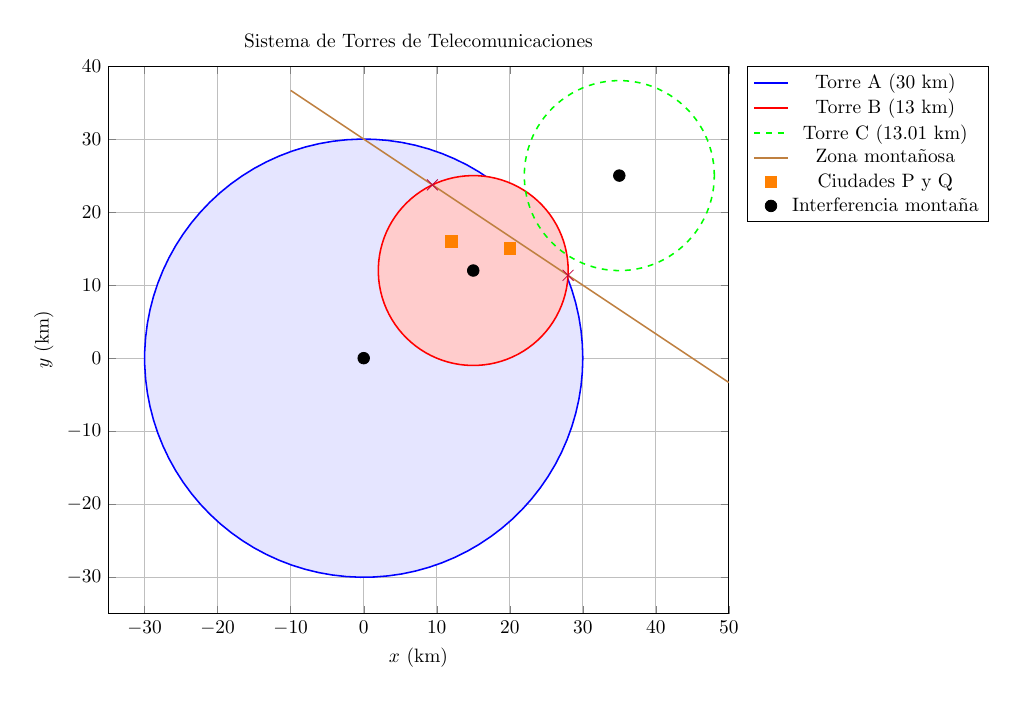
\begin{tikzpicture}[scale=0.7]
\begin{axis}[
    axis equal image,
    width=1.2\textwidth,
    height=0.95\textwidth,
    xlabel={$x$ (km)},
    ylabel={$y$ (km)},
    grid=major,
    xmin=-35, xmax=50,
    ymin=-35, ymax=40,
    title={Sistema de Torres de Telecomunicaciones},
    legend pos=outer north east
]
% Torre A
\addplot[domain=0:360, samples=100, thick, blue, fill=blue!10, variable=\t]
    ({30*cos(\t)}, {30*sin(\t)});
\addlegendentry{Torre A (30 km)}

% Torre B
\addplot[domain=0:360, samples=100, thick, red, fill=red!20, variable=\t]
    ({15 + 13*cos(\t)}, {12 + 13*sin(\t)});
\addlegendentry{Torre B (13 km)}

% Torre C (propuesta)
\addplot[domain=0:360, samples=100, thick, green, dashed, variable=\t]
    ({35 + 13.01*cos(\t)}, {25 + 13.01*sin(\t)});
\addlegendentry{Torre C (13.01 km)}

% Zona montañosa
\addplot[domain=-10:50, thick, brown] {(90 - 2*x)/3};
\addlegendentry{Zona montañosa}

% Ciudades
\addplot[only marks, mark=square*, mark size=3pt, orange] coordinates {(12, 16) (20, 15)};
\addlegendentry{Ciudades P y Q}

% Centros de torres
\addplot[only marks, mark=*, mark size=3pt, black] coordinates {(0, 0) (15, 12) (35, 25)};

% Puntos de intersección
\addplot[only marks, mark=x, mark size=4pt, purple] coordinates {(27.98, 11.35) (9.40, 23.73)};
\addlegendentry{Interferencia montaña}
\end{axis}
\end{tikzpicture}
\end{center}

\textbf{Respuestas finales:}
\begin{itemize}
    \item a) Torre B: Centro \boxed{C_B(15, 12) \text{ km}}, Radio \boxed{r_B = 13 \text{ km}}
    \item b) Área compartida: \boxed{169\pi \approx 531.10 \text{ km}^2}
    \item c) Puntos de corte con montaña: \boxed{(27.98, 11.35) \text{ y } (9.40, 23.73) \text{ km}}
    \item d) Radio mínimo Torre C: \boxed{r_C = 13.01 \text{ km}}
\end{itemize}
\end{solucion}

\begin{ejercicio}[title={Ejercicio Inverso 4: El Diseñador de Juegos y la Mecánica de Colisiones}]
En un videojuego de billar espacial, las bolas se mueven en un tablero bidimensional. El diseñador de juegos, Carlos Méndez, está programando la física de colisiones con las siguientes especificaciones:

\begin{itemize}
    \item Bola Blanca: Se mueve por la trayectoria rectilínea $y = 2x - 10$ (unidades en píxeles).
    \item Bola Objetivo: Circunferencia con centro en $(15, 8)$ y radio 4 píxeles.
    \item Agujero Negro: Zona circular peligrosa con ecuación $x^2 + y^2 - 6x + 8y - 75 = 0$.
    \item Bola de Poder: Aparece en una circunferencia que pasa por los puntos $(5, 2)$, $(13, 4)$ y $(9, 10)$.
\end{itemize}

El sistema debe calcular:
\begin{enumerate}[a)]
    \item Los puntos exactos donde la Bola Blanca impactará la Bola Objetivo (si es que la toca).
    \item El centro y radio del Agujero Negro, y si la trayectoria de la Bola Blanca lo atraviesa.
    \item La ecuación de la circunferencia donde aparece la Bola de Poder.
    \item Si existe algún punto seguro donde las tres circunferencias (Objetivo, Agujero Negro y Poder) estén a exactamente la misma distancia.
\end{enumerate}
\end{ejercicio}

\begin{solucion}[title={Solución Ejercicio Inverso 4}]
\textbf{Parte a) Puntos de impacto Bola Blanca con Bola Objetivo}

\textbf{Paso 1:} Trayectoria de la Bola Blanca: $y = 2x - 10$
Bola Objetivo: $(x - 15)^2 + (y - 8)^2 = 16$

\textbf{Paso 2:} Sustituyendo la trayectoria en la circunferencia:
$$(x - 15)^2 + (2x - 10 - 8)^2 = 16$$
$$(x - 15)^2 + (2x - 18)^2 = 16$$
$$x^2 - 30x + 225 + 4x^2 - 72x + 324 = 16$$
$$5x^2 - 102x + 533 = 0$$

\textbf{Paso 3:} Aplicando la fórmula cuadrática:
$$x = \frac{102 \pm \sqrt{10404 - 10660}}{10} = \frac{102 \pm \sqrt{-256}}{10}$$

Como el discriminante es negativo, NO hay puntos reales de intersección.
La Bola Blanca NO impacta la Bola Objetivo.

\textbf{Verificación:} Calculemos la distancia mínima del centro $(15, 8)$ a la recta $2x - y - 10 = 0$:
$$d = \frac{|2(15) - 8 - 10|}{\sqrt{4 + 1}} = \frac{|30 - 18|}{\sqrt{5}} = \frac{12}{\sqrt{5}} = \frac{12\sqrt{5}}{5} \approx 5.37$$

Como $d = 5.37 > r = 4$, confirma que no hay intersección.

\textbf{Parte b) Agujero Negro y trayectoria}

\textbf{Paso 1:} Completar cuadrados para $x^2 + y^2 - 6x + 8y - 75 = 0$:
$$(x^2 - 6x) + (y^2 + 8y) = 75$$
$$(x^2 - 6x + 9) - 9 + (y^2 + 8y + 16) - 16 = 75$$
$$(x - 3)^2 + (y + 4)^2 = 100$$

Centro del Agujero Negro: $C_{AN}(3, -4)$
Radio: $r_{AN} = 10$ píxeles

\textbf{Paso 2:} Verificar si la trayectoria atraviesa el Agujero Negro.
Distancia del centro $(3, -4)$ a la recta $2x - y - 10 = 0$:
$$d = \frac{|2(3) - (-4) - 10|}{\sqrt{5}} = \frac{|6 + 4 - 10|}{\sqrt{5}} = \frac{0}{\sqrt{5}} = 0$$

¡La recta pasa por el centro del Agujero Negro! Definitivamente lo atraviesa.

\textbf{Paso 3:} Puntos de entrada y salida:
Sustituyendo $y = 2x - 10$ en $(x - 3)^2 + (y + 4)^2 = 100$:
$$(x - 3)^2 + (2x - 10 + 4)^2 = 100$$
$$(x - 3)^2 + (2x - 6)^2 = 100$$
$$x^2 - 6x + 9 + 4x^2 - 24x + 36 = 100$$
$$5x^2 - 30x - 55 = 0$$
$$x^2 - 6x - 11 = 0$$
$$x = \frac{6 \pm \sqrt{36 + 44}}{2} = \frac{6 \pm \sqrt{80}}{2} = 3 \pm 2\sqrt{5}$$

Puntos: $(3 - 2\sqrt{5}, -4 - 4\sqrt{5})$ y $(3 + 2\sqrt{5}, -4 + 4\sqrt{5})$
Aproximadamente: $(-1.47, -18.94)$ y $(7.47, 4.94)$

\textbf{Parte c) Circunferencia de la Bola de Poder}

\textbf{Paso 1:} Usando los puntos $(5, 2)$, $(13, 4)$ y $(9, 10)$.
Ecuación general: $x^2 + y^2 + Dx + Ey + F = 0$

\textbf{Paso 2:} Sistema de ecuaciones:
Para $(5, 2)$: $25 + 4 + 5D + 2E + F = 0 \Rightarrow 5D + 2E + F = -29$
Para $(13, 4)$: $169 + 16 + 13D + 4E + F = 0 \Rightarrow 13D + 4E + F = -185$
Para $(9, 10)$: $81 + 100 + 9D + 10E + F = 0 \Rightarrow 9D + 10E + F = -181$

\textbf{Paso 3:} Resolviendo por eliminación:
De ecuaciones 1 y 2: $8D + 2E = -156 \Rightarrow 4D + E = -78$
De ecuaciones 1 y 3: $4D + 8E = -152 \Rightarrow D + 2E = -38$

De estas dos: $3D - E = -40$ y $D + 2E = -38$
Resolviendo: $D = -18$, $E = -10$, $F = 91$

\textbf{Paso 4:} Ecuación de la Bola de Poder:
$$x^2 + y^2 - 18x - 10y + 91 = 0$$

Centro: $C_{BP}(9, 5)$
Radio: $r_{BP} = \sqrt{81 + 25 - 91} = \sqrt{15}$ píxeles

\textbf{Parte d) Punto equidistante de las tres circunferencias}

\textbf{Paso 1:} Buscamos punto $P(x, y)$ tal que:
- Distancia a Bola Objetivo $(15, 8)$, radio 4
- Distancia a Agujero Negro $(3, -4)$, radio 10
- Distancia a Bola de Poder $(9, 5)$, radio $\sqrt{15}$

\textbf{Paso 2:} Las distancias a las circunferencias (no a los centros) deben ser iguales:
$$|\sqrt{(x-15)^2 + (y-8)^2} - 4| = |\sqrt{(x-3)^2 + (y+4)^2} - 10| = |\sqrt{(x-9)^2 + (y-5)^2} - \sqrt{15}|$$

\textbf{Paso 3:} Este es el centro radical de las tres circunferencias.
Eje radical de Objetivo y Agujero Negro:
$$(x-15)^2 + (y-8)^2 - 16 = (x-3)^2 + (y+4)^2 - 100$$
$$-30x + 225 - 16y + 64 - 16 = -6x + 9 + 8y + 16 - 100$$
$$-24x - 24y + 348 = 0$$
$$x + y = 14.5$$

Eje radical de Objetivo y Poder:
$$(x-15)^2 + (y-8)^2 - 16 = (x-9)^2 + (y-5)^2 - 15$$
$$-30x + 225 - 16y + 64 - 16 = -18x + 81 - 10y + 25 - 15$$
$$-12x - 6y + 182 = 0$$
$$2x + y = 30.33$$

\textbf{Paso 4:} Resolviendo el sistema:
De $x + y = 14.5$ y $2x + y = 30.33$:
$$x = 15.83$$
$$y = -1.33$$

Punto equidistante: $(15.83, -1.33)$ píxeles

\textbf{Verificación gráfica:}

\begin{center}
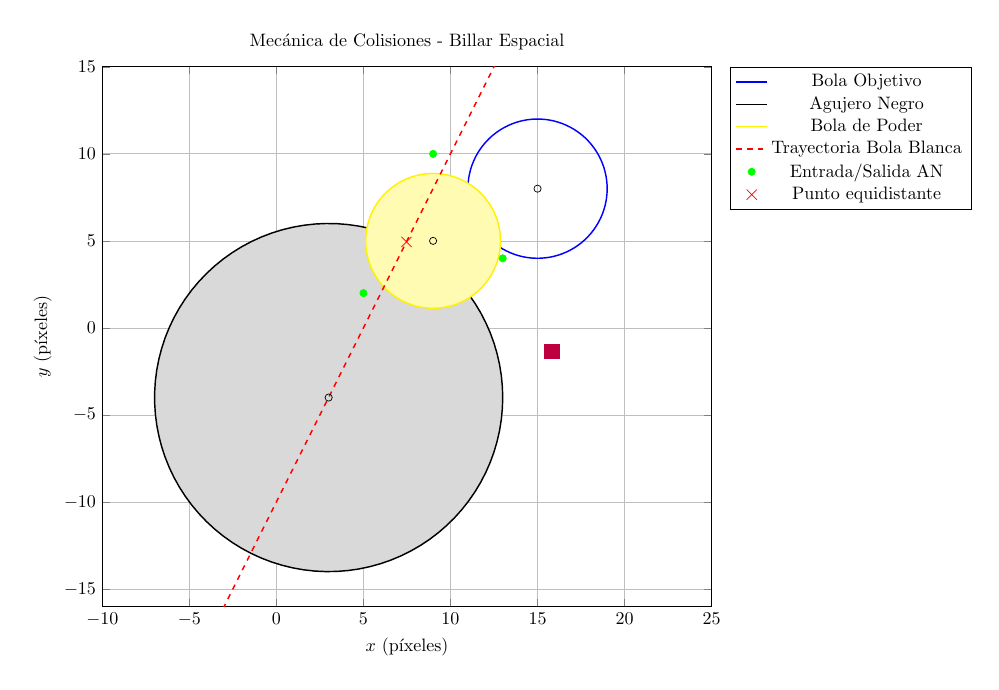
\begin{tikzpicture}[scale=0.65]
\begin{axis}[
    axis equal image,
    width=1.3\textwidth,
    height=1.0\textwidth,
    xlabel={$x$ (píxeles)},
    ylabel={$y$ (píxeles)},
    grid=major,
    xmin=-10, xmax=25,
    ymin=-16, ymax=15,
    title={Mecánica de Colisiones - Billar Espacial},
    legend pos=outer north east
]
% Bola Objetivo
\addplot[domain=0:360, samples=100, thick, blue, variable=\t]
    ({15 + 4*cos(\t)}, {8 + 4*sin(\t)});
\addlegendentry{Bola Objetivo}

% Agujero Negro
\addplot[domain=0:360, samples=100, thick, black, fill=gray!30, variable=\t]
    ({3 + 10*cos(\t)}, {-4 + 10*sin(\t)});
\addlegendentry{Agujero Negro}

% Bola de Poder
\addplot[domain=0:360, samples=100, thick, yellow, fill=yellow!30, variable=\t]
    ({9 + sqrt(15)*cos(\t)}, {5 + sqrt(15)*sin(\t)});
\addlegendentry{Bola de Poder}

% Trayectoria de la Bola Blanca
\addplot[domain=-10:25, thick, red, dashed] {2*x - 10};
\addlegendentry{Trayectoria Bola Blanca}

% Puntos de formación de la Bola de Poder
\addplot[only marks, mark=*, mark size=2pt, green] coordinates {(5, 2) (13, 4) (9, 10)};

% Puntos de cruce con Agujero Negro
\addplot[only marks, mark=x, mark size=4pt, red] coordinates {(-1.47, -18.94) (7.47, 4.94)};
\addlegendentry{Entrada/Salida AN}

% Punto equidistante
\addplot[only marks, mark=square*, mark size=4pt, purple] coordinates {(15.83, -1.33)};
\addlegendentry{Punto equidistante}

% Centros
\addplot[only marks, mark=o, mark size=2pt, black] coordinates {(15, 8) (3, -4) (9, 5)};
\end{axis}
\end{tikzpicture}
\end{center}

\textbf{Respuestas finales:}
\begin{itemize}
    \item a) La Bola Blanca \boxed{\text{NO impacta}} la Bola Objetivo (distancia mínima 5.37 píxeles)
    \item b) Agujero Negro: Centro \boxed{(3, -4)}, Radio \boxed{10 \text{ píxeles}}. La trayectoria \boxed{\text{SÍ lo atraviesa}} por su centro
    \item c) Bola de Poder: \boxed{x^2 + y^2 - 18x - 10y + 91 = 0}, Centro \boxed{(9, 5)}, Radio \boxed{\sqrt{15} \text{ píxeles}}
    \item d) Punto equidistante: \boxed{(15.83, -1.33) \text{ píxeles}}
\end{itemize}
\end{solucion}